\section{AIT and Kolmogorov complexity}
%%%%%%%%%%%%%%%%%%%%%%%%%%%%%%%%%%%%%%%%%%%%%%%%%%%%%%%%%%%%%%%%%%%%%%
\begin{frame}[label=intro3]{Kolmogorov complexity ($\Ko$) I}
 We can think of agents as physical systems, and in turn,  of physical systems as dynamical systems calculating (effectively computable) functions.   This allows us to analyze agents from the standpoint of computation theory.
 \begin{alertblock}{Warning: Computation is a mathematical concept (Turing machine)}
The use of computational framework  in KT should not be construed to mean that the brain is literally a physical von Neumann computer (such as a laptop).
\end{alertblock}\vfill 
 
A computational perspective  leads us directly into algorithmic information theory (AIT) and its central concept: 


\begin{definition}[Kolmogorov complexity  of a dataset $\Ko$]
The length of the shortest program capable of generating  the dataset \citep{Kolomgorov1965,Cover:2006aa}.  
\end{definition} \vfill

\end{frame}


%%%%%%%%%%%%%%%%%%%%%%%%%%%%%%%%%%%%%%%%%%%%%%%%%%%%%%%%%%%%%%%%%%%%%%
\begin{frame}[label=intro3]{Kolmogorov complexity ($\Ko$) II}
 \begin{center}%\includegraphics[height=1.2cm]{COPL}%
  %\hspace{2cm}
  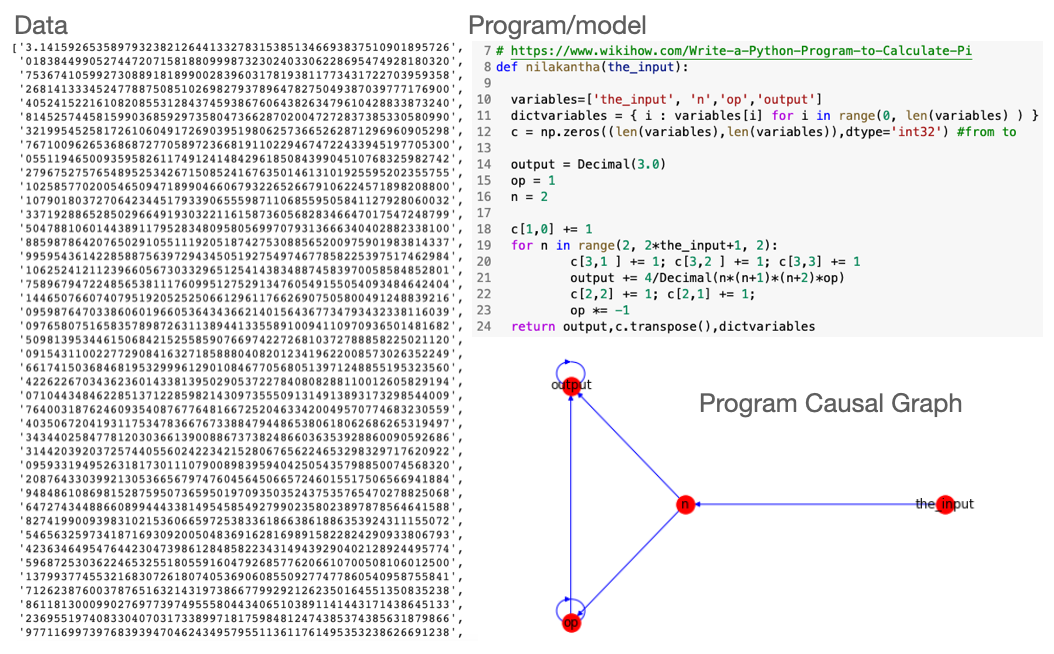
\includegraphics[height=7.2cm]{img/pi.png}
  \end{center}
\end{frame}

%%%%%%%%%%%%%%%%%%%%%%%%%%%%%%%%%%%%%%%%%%%%%%%%%%%%%%%%%%%%%%%%%%%%%%
\begin{frame}[label=intro3]{Mutual algorithmic information ($\mathcal M$)}
With 
\K at hand, we can define an algorithmic version of mutual information we will also need: \vfill

\begin{definition}[Mutual algorithmic information complexity  $\mathcal M$]
The {\em mutual algorithmic information  $\mathcal M(x:y)$ between two strings $x$ and $y$, is given by  }
$$
\mathcal M(x \!:\!y) = \Ko(x) +\Ko(y)- \Ko(x,y)
$$
%where $\Ko(y|x)$ is the complexity of the string $y$ if the computer has access to $x$ 
\citep{Li:1997aa, Grunwald:2004aa}.  
\end{definition}
\end{frame}

%%%%%%%%%%%%%%%%%%%%%%%%%%%%%%%%%%%%%%%%%%%%%%%%%%%%%%%%%%%%%%%%%%%%%%
\begin{frame}[label=ladila]{Hierarchy class \citep{Fitch2014}}
Not all programming languages are equal. Recurrence is needed for Turing completeness, for example. 
 \begin{center}%\includegraphics[height=1.2cm]{COPL}%
  %\hspace{2cm}
  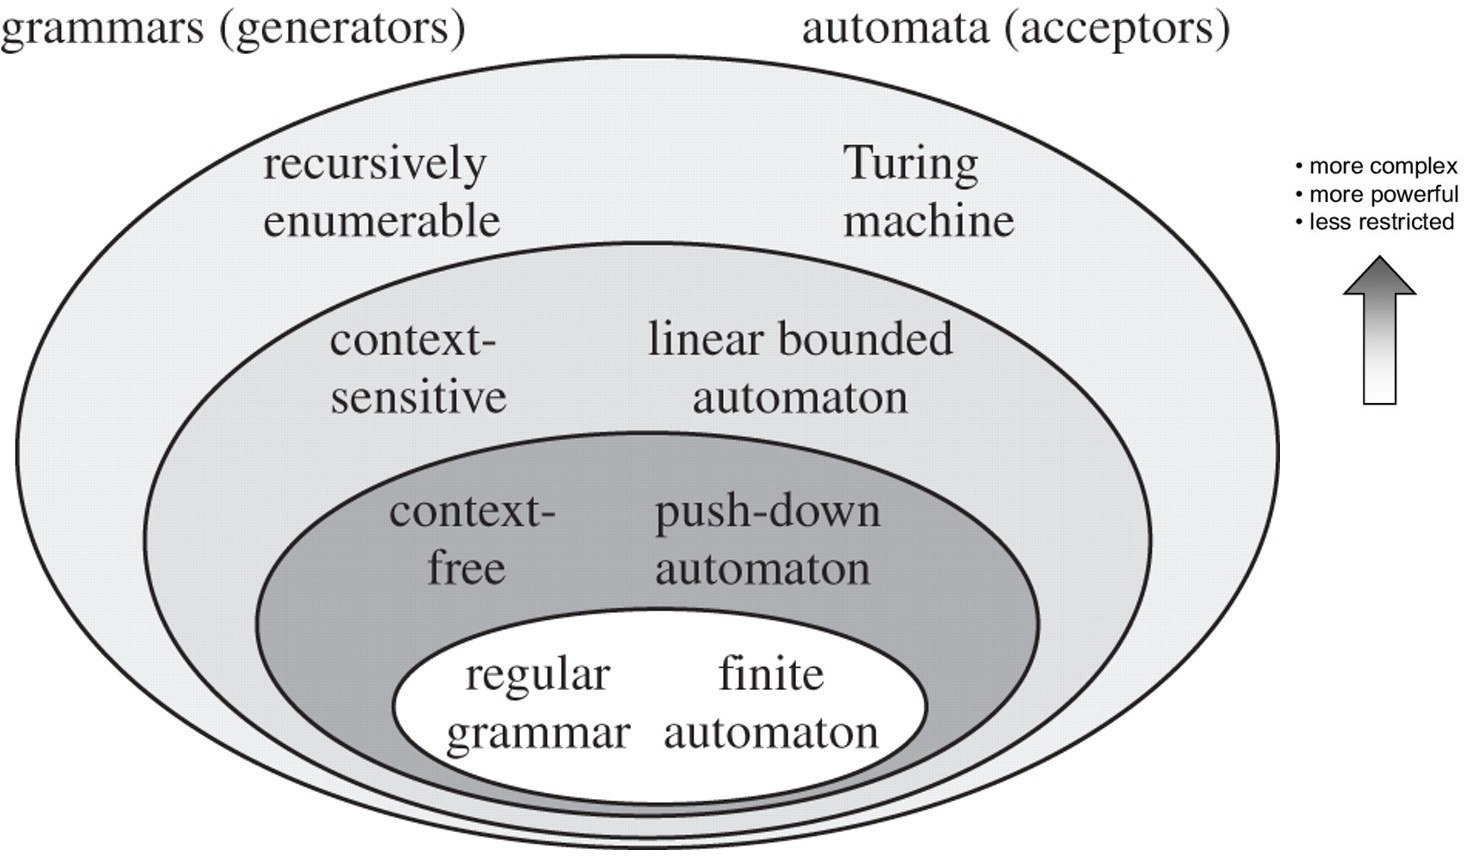
\includegraphics[height=5.5cm]{img/chomsky.jpg}
  \end{center}
\end{frame}

%%%%%%%%%%%%%%%%%%%%%%%%%%%%%%%%%%%%%%%%%%%%%%%%%%%%%%%%%%%%%%%%%%%%%%
\begin{frame}[label=ladila]{Model I}
The notion of {\bf model} is central in KT and other theories of consciousness. \vfill

 %With AIT as a basis, we can now define what a  model is and an optimal model. \vfill 
 
 \begin{definition}[Model]
 A  model  of a dataset is any program that generates the dataset. 
 \end{definition}
Models may differ in two ways: they may implement different functions, or they may implement the same function in different ways. Both aspects matter here.  We focus on those that implement the right functions succinctly. \vfill 
 
\begin{definition}[Optimal model]
The optimal model of a dataset is the shortest program that generates (or, equivalently, compresses) the dataset.
\end{definition}
\end{frame}


%%%%%%%%%%%%%%%%%%%%%%%%%%%%%%%%%%%%%%%%%%%%%%%%%%%%%%%%%%%%%%%%%%%%%%
\begin{frame}[label=ladila]{Model II}

An {\bf optimal model needs to capture and exploit all the structure in the dataset}---and nothing else. In some sense, the {\em structure of the model can be described by the group of symmetries of the dataset}  \citep{Ruffini:2016ad}. 
 \begin{center}%\includegraphics[height=1.2cm]{COPL}%
  %\hspace{2cm}
  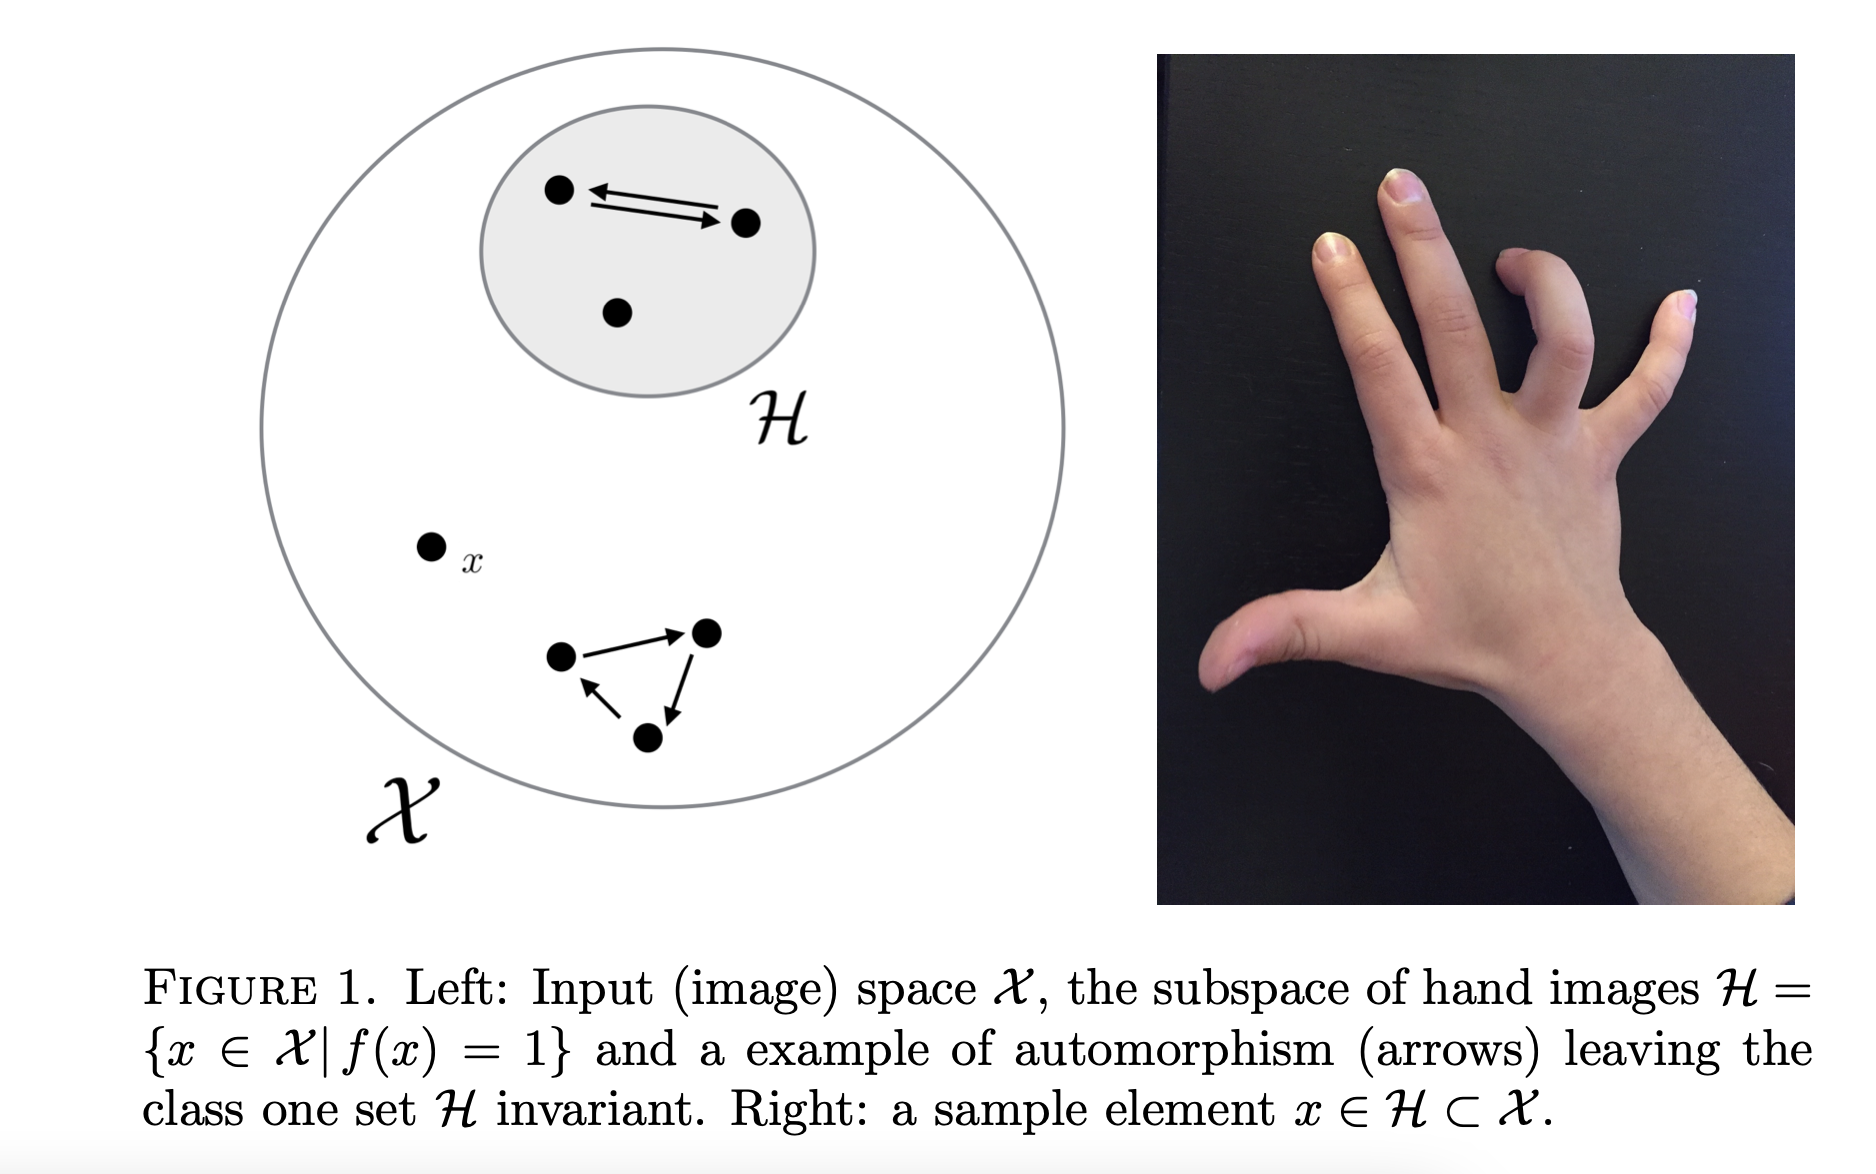
\includegraphics[height=4cm]{img/hand2.png}
  \end{center}
  
Suppose we are given a stack of images of a hand, e.g., from the frames of a movie of a moving hand  created using a generating function,
$y = f(\theta)$, where $y$ is the image in a frame and $\theta$ a parametrization of the hand image and view.
\end{frame}

\begin{frame}[label=ladila]{Model III}
 \begin{center}%\includegraphics[height=1.2cm]{COPL}%
  %\hspace{2cm}
  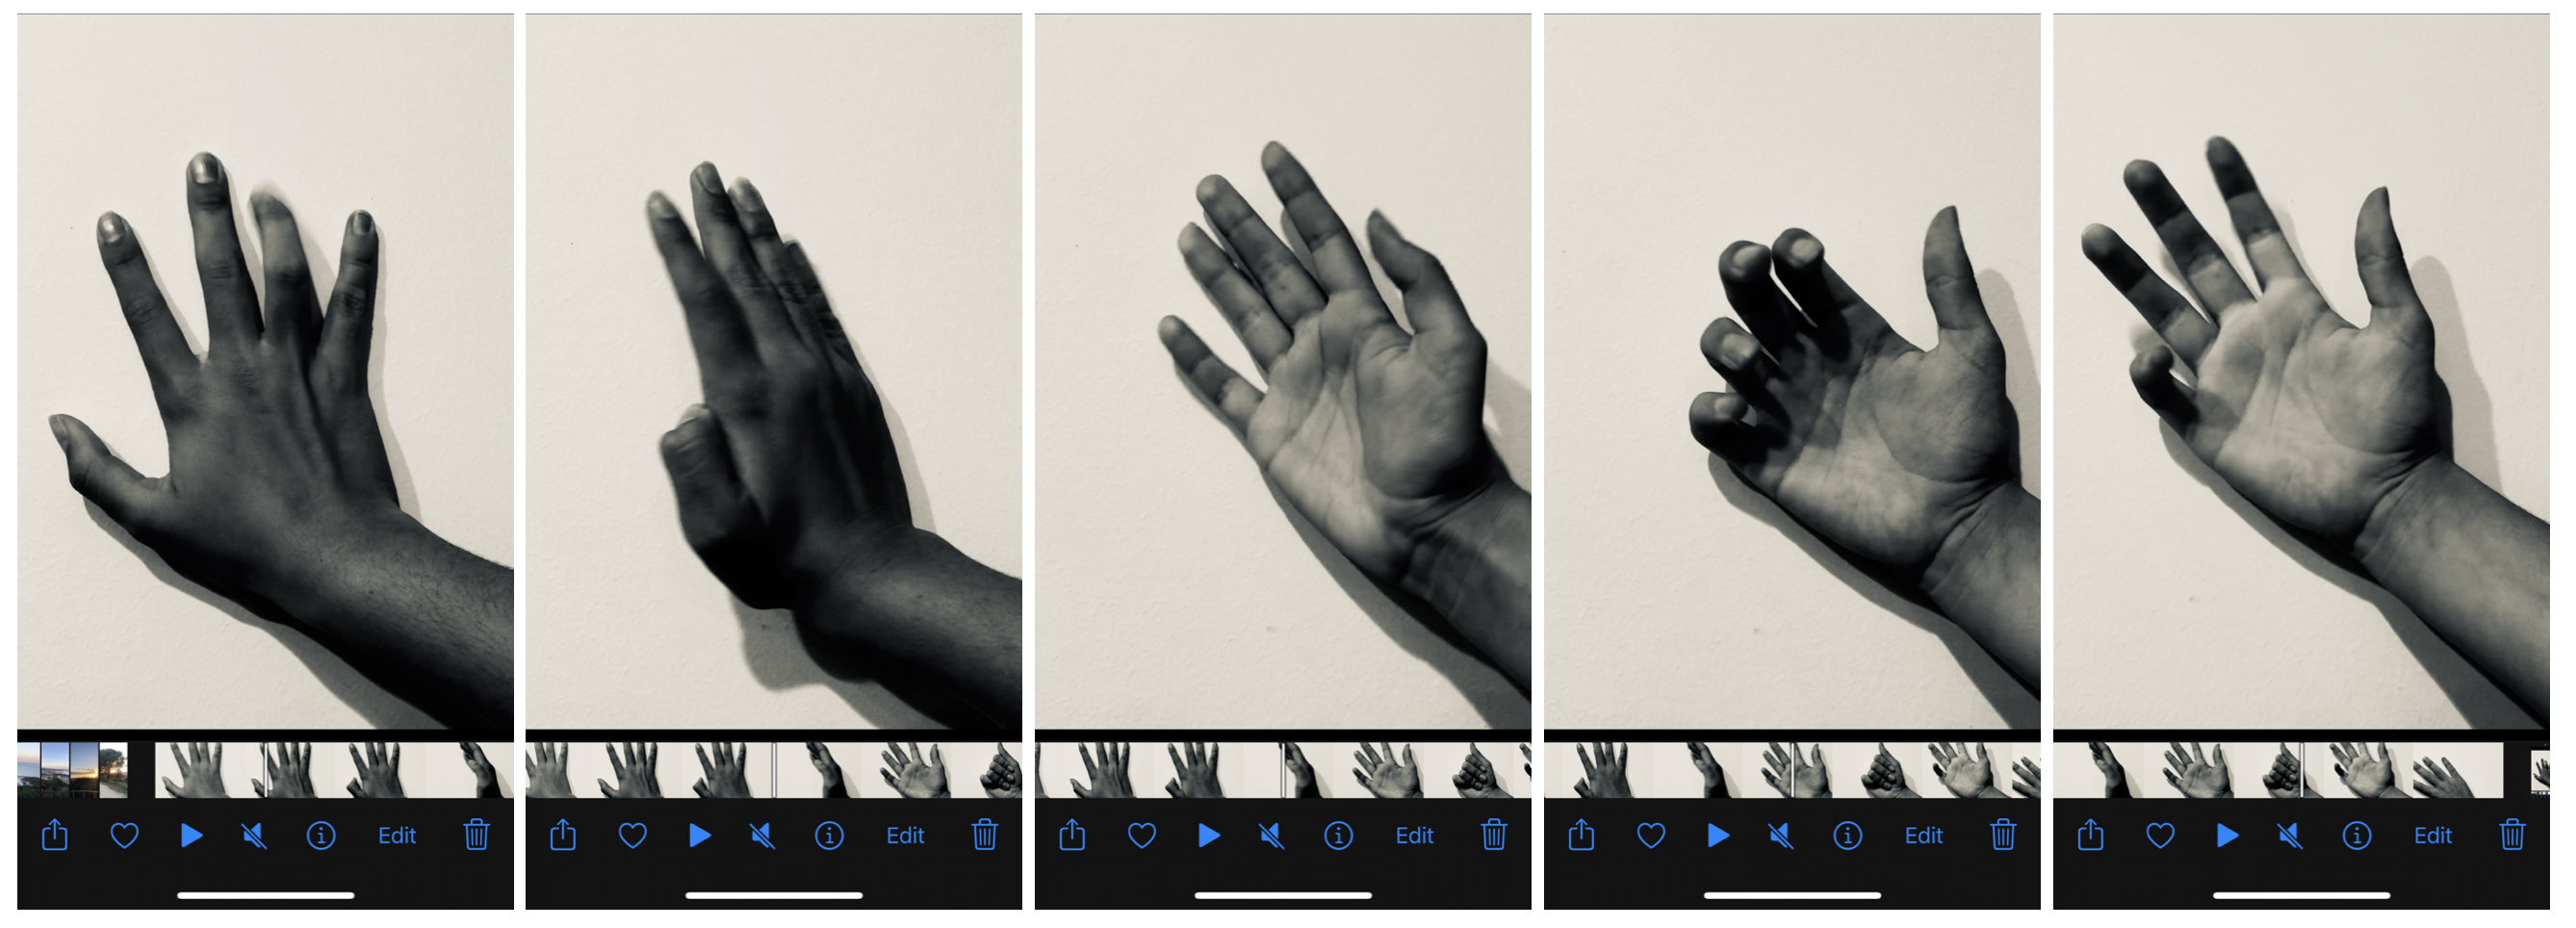
\includegraphics[height=5cm]{img/hands.png}
  \end{center}
  The structure of the dataset is encapsulated by the minimal program that encodes the function $y=f(x)$---the {\em invariant} object.  %The {\bf symmetries} of the dataset are parametrized by $\theta$, and they are symmetries in the sense that if $\theta\rightarrow \theta'$ and $y\rightarrow y'$, then the equation $y'-f(\theta') =0 $ holds true.
\end{frame}



%%%%%%%%%%%%%%%%%%%%%%%%%%%%%%%%%%%%%%%%%%%%%%%%%%%%%%%%%%%%%%%%%%%%%%
\begin{frame}[label=ladila]{Why are ``good models'' good?}

The rationale for the importance of compressive (succinct) models is discussed in detail in \cite{Ruffini:2007aa,Ruffini:2009aa,Ruffini2017}.  Rephrase of the principle of Occam’s Razor: {\em
one should not increase, beyond what is necessary, the number of entities required to explain anything.}  Ok, but why?\vfill

The universe appears to be simple. Simple rules can create apparent complexity.\vfill


Simple data generators are more likely if the universe rules are drawn from a random algorithmic bingo (Solomonoff's prior). \vfill

Simple models are unbiased and generalize better (Occam, Laplace, Jaynes). \vfill

They are easier to construct,  store,  and reuse for model-building. \vfill


%Simple models can be maximally powerful (Turing complete)

\end{frame}